
\section{Aurora I}
\label{section:aurora_1}
\begin{frame}%STARTCONTENT

\begin{figure}
    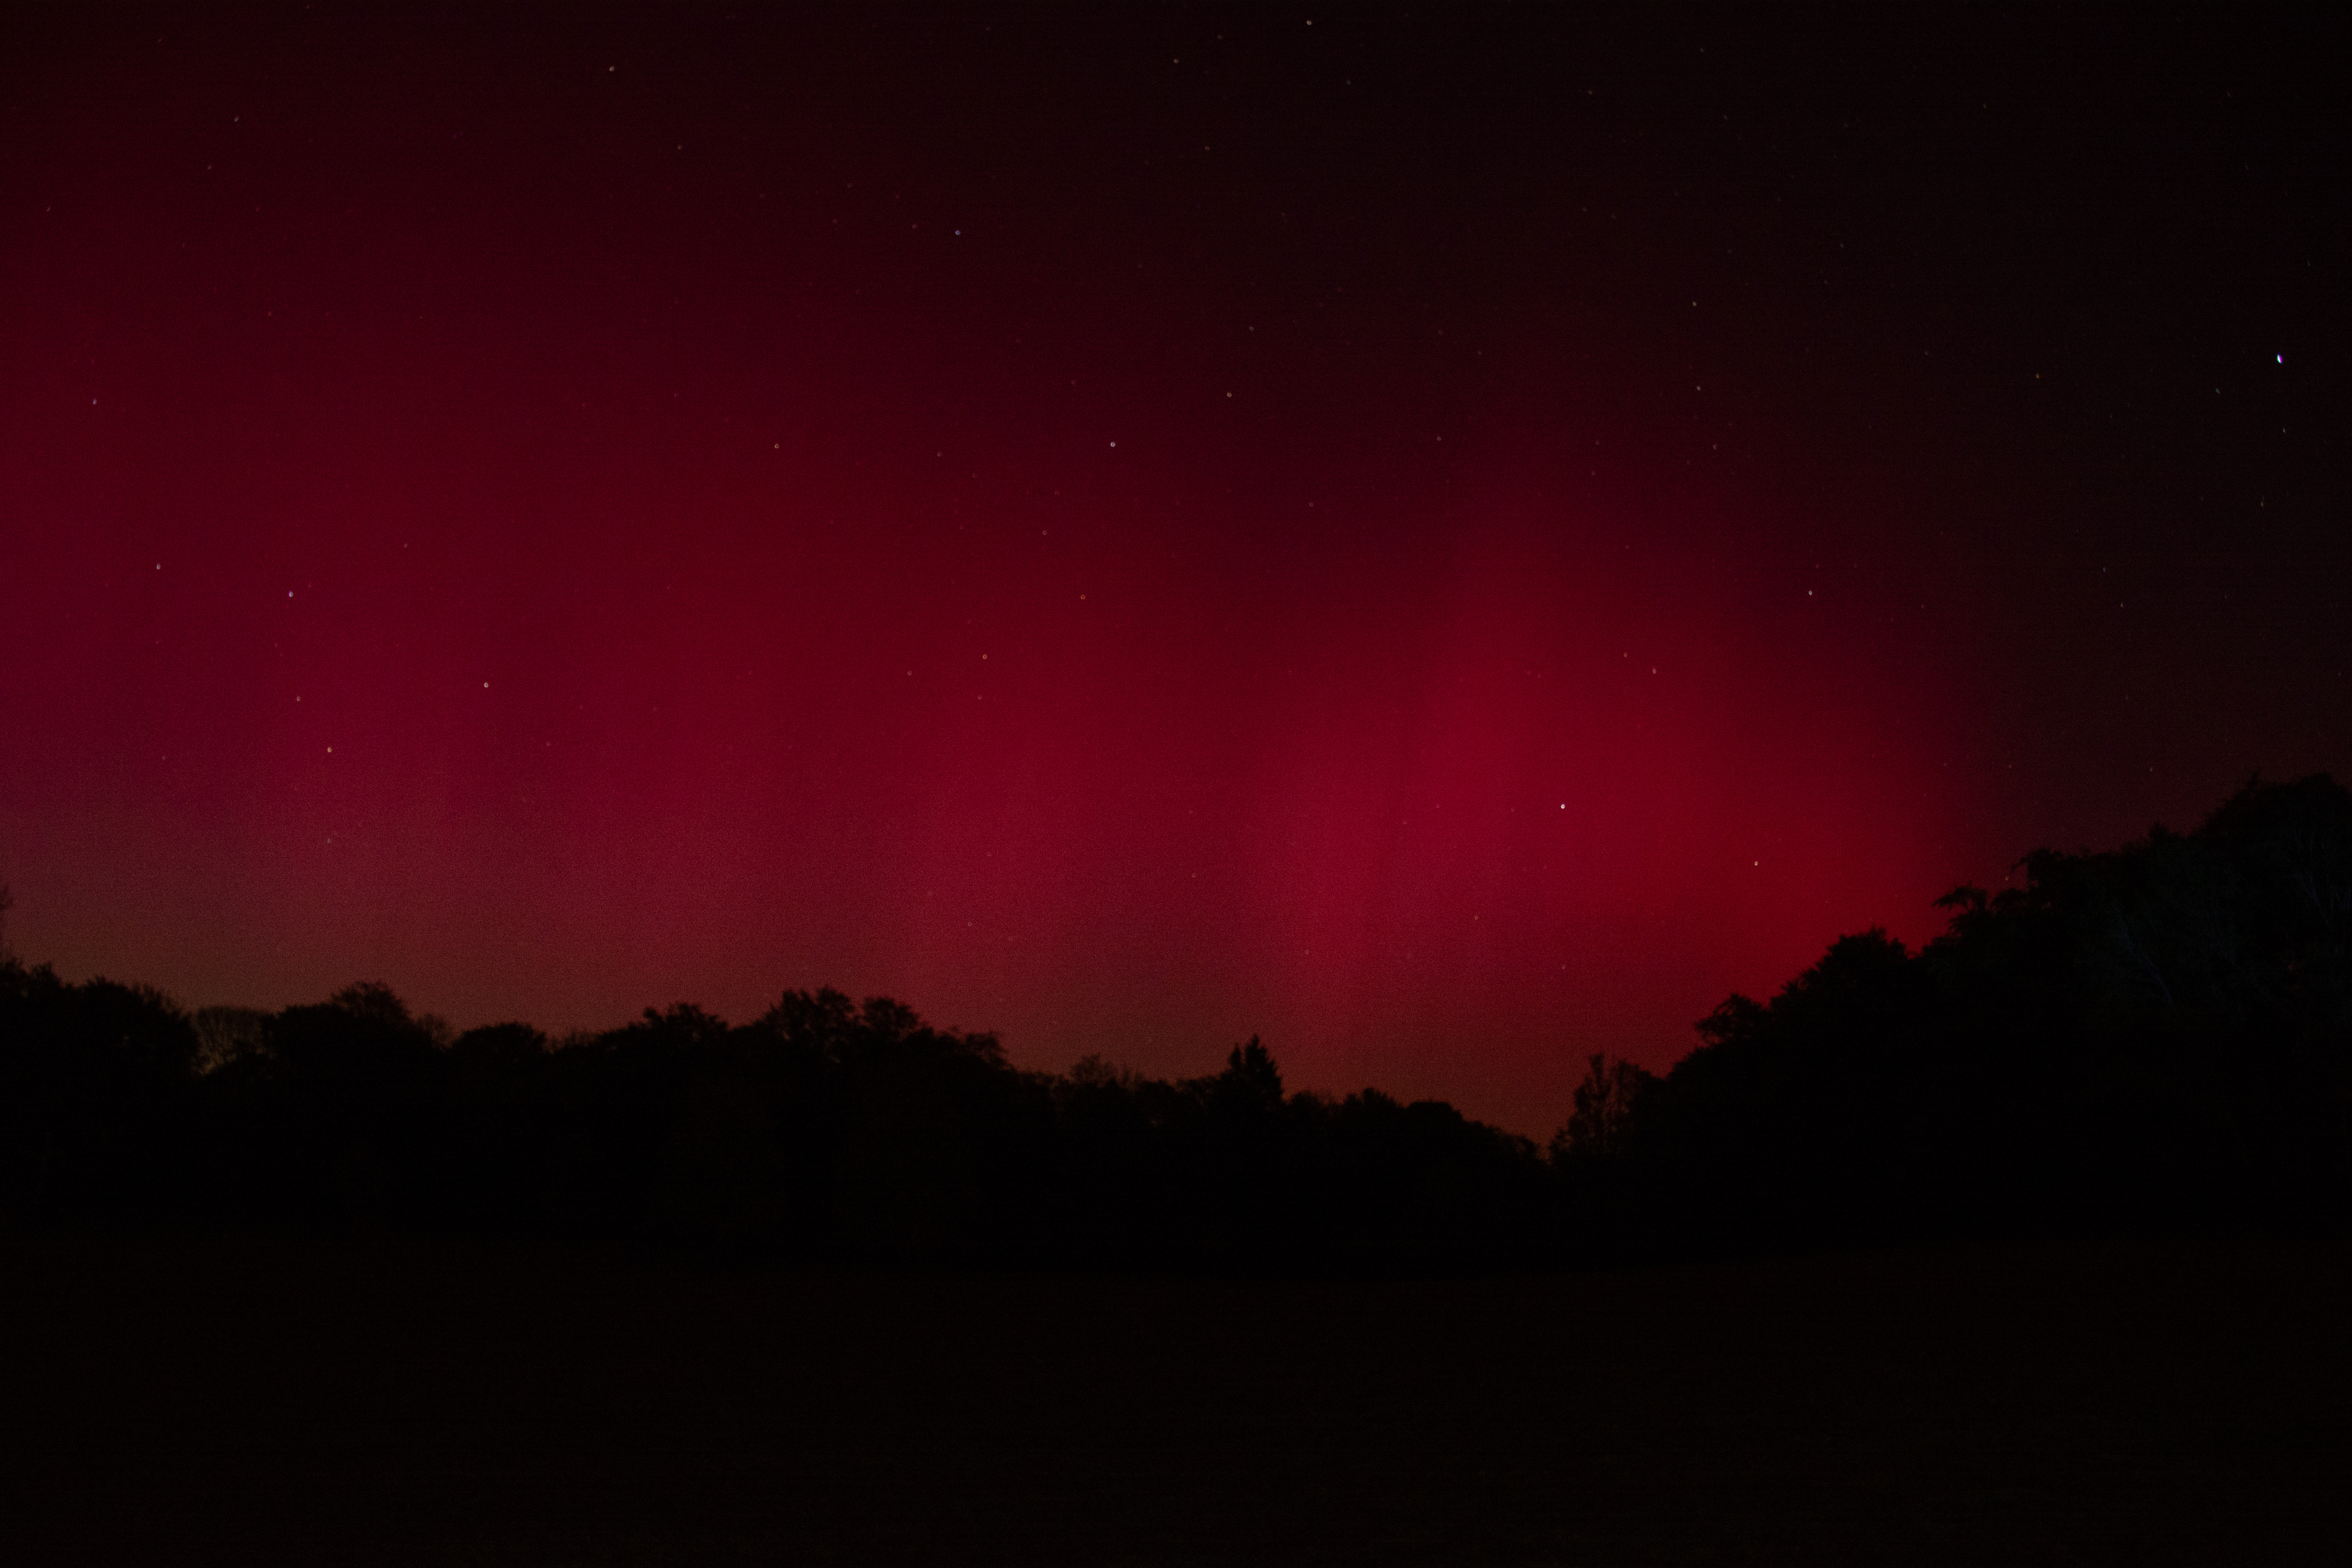
\includegraphics[width=0.85\textwidth]{foto/217}
    \caption{\scriptsize Aurora am Notfunk Ausbildungswochenende im Mai 2024}
    \label{e_aurora}
\end{figure}
\end{frame}

\begin{frame}\begin{itemize}
  \item Aurora- oder Polarlichterscheinung in ca. \qtyrange{90}{200}{\kilo\metre} Höhe
  \item Hauptsächlich über magnetischen Nord- und Südpol
  \item Sauerstoff- und Stickstoffatome werden vom Sonnenwind angeregt oder ionisiert
  \item Sonnenwind: Elektrisch geladene Teilchen
  \item Bei Sonneneruptionen besonders stark
  \end{itemize}
\end{frame}

\begin{frame}
\frametitle{Aurora und Amateurfunk}
\begin{itemize}
  \item Funkwellen können sich an ionisierten Sauerstoff- und Stickstoffatomen brechen
  \item Insbesondere für VHF-DX-Verbindungen nutzbar
  \item Sprache nur schlecht nutzbar (große Bandbreite)
  \item Für CW und Digimodes brauchbar
  \item Rapport: für T wird \enquote{A} vergeben, da Ton rau und schwankend ist 
  \end{itemize}
\end{frame}

\begin{frame}
\only<1>{
\begin{QQuestion}{EH305}{Wie wird ein Aurora-Signal in Morsetelegrafie beurteilt?}{Es wird beurteilt mit R und T, weil die Signalstärke stark schwankt.}
{Es wird beurteilt mit R, S und T, da Aurora-Verbindungen überwiegend in CW getätigt werden.}
{Es wird beurteilt mit R, S und \glqq A\grqq{} für Aurora, da der Ton bei Aurora sehr rau ist und nicht beurteilt werden kann.}
{Es wird beurteilt mit R, S, T und \glqq A\grqq{} für Aurora.}
\end{QQuestion}

}
\only<2>{
\begin{QQuestion}{EH305}{Wie wird ein Aurora-Signal in Morsetelegrafie beurteilt?}{Es wird beurteilt mit R und T, weil die Signalstärke stark schwankt.}
{Es wird beurteilt mit R, S und T, da Aurora-Verbindungen überwiegend in CW getätigt werden.}
{\textbf{\textcolor{DARCgreen}{Es wird beurteilt mit R, S und \glqq A\grqq{} für Aurora, da der Ton bei Aurora sehr rau ist und nicht beurteilt werden kann.}}}
{Es wird beurteilt mit R, S, T und \glqq A\grqq{} für Aurora.}
\end{QQuestion}

}
\end{frame}%ENDCONTENT
